\documentclass{standalone}
\usepackage[dvipsnames]{xcolor}
\usepackage{tikz}
\usetikzlibrary{shapes}

\begin{document}
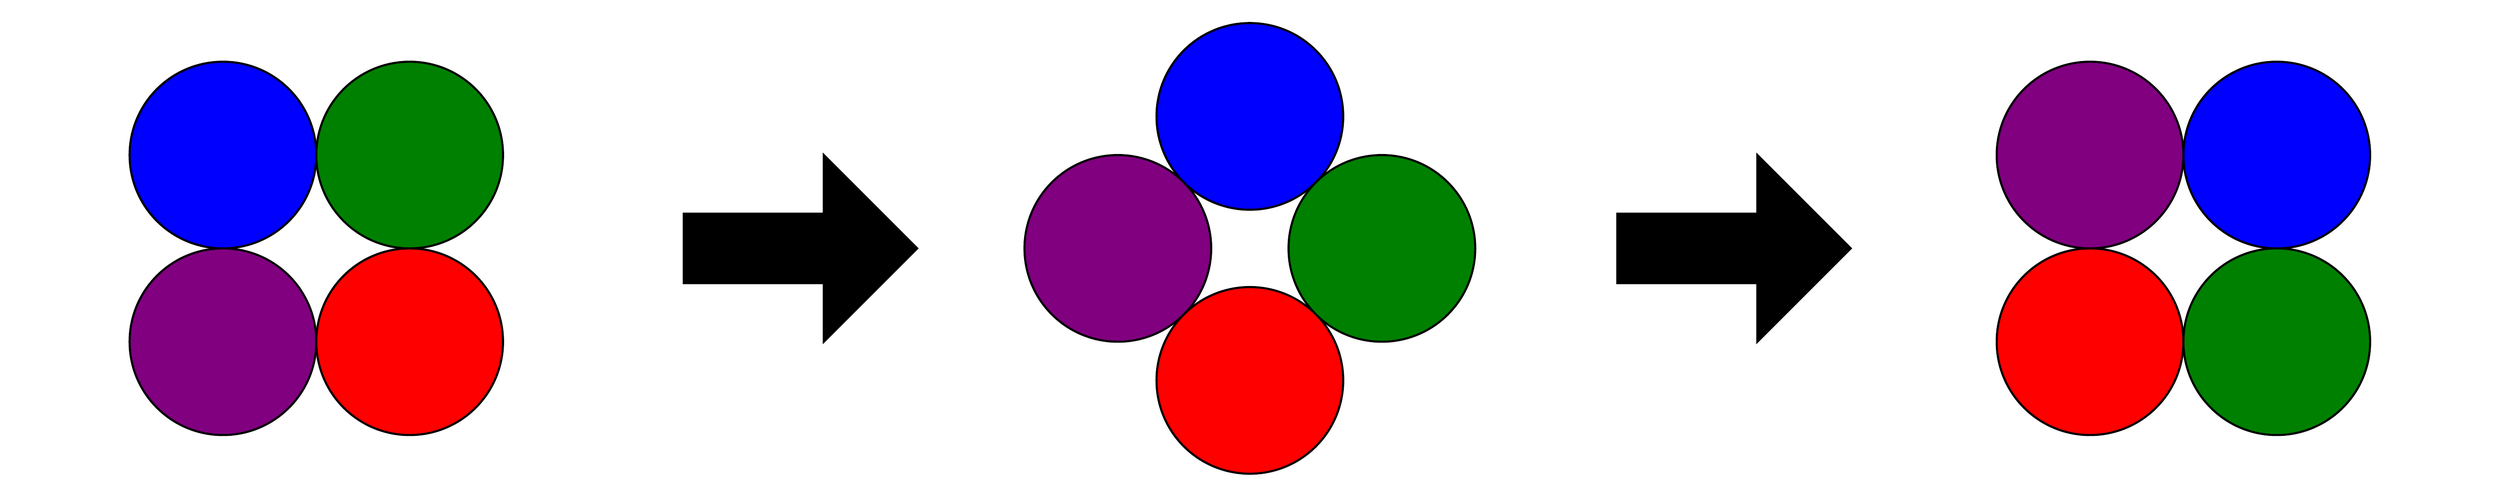
\begin{tikzpicture}[x=1in, y=1in]
\node[draw, circle, ultra thick, inner sep=0pt, minimum size=2in, fill=Blue] () at (1,0) {};
\node[draw, circle, ultra thick, inner sep=0pt, minimum size=2in, fill=Green] () at (3,0) {};
\node[draw, circle, ultra thick, inner sep=0pt, minimum size=2in, fill=Purple] () at (1,-2) {};
\node[draw, circle, ultra thick, inner sep=0pt, minimum size=2in, fill=Red] () at (3,-2) {};

\node[draw, single arrow, ultra thick, fill=black, inner sep=0pt, minimum height=2.5in, minimum width=2in] () at (7,-1) {\phantom{M}};

\node[draw, circle, ultra thick, inner sep=0pt, minimum size=2in, fill=Blue, rotate around={-45:(1,-1)}] () at (11,0) {};
\node[draw, circle, ultra thick, inner sep=0pt, minimum size=2in, fill=Green, rotate around={-45:(-1,-1)}] () at (13,0) {};
\node[draw, circle, ultra thick, inner sep=0pt, minimum size=2in, fill=Purple, rotate around={-45:(1,1)}] () at (11,-2) {};
\node[draw, circle, ultra thick, inner sep=0pt, minimum size=2in, fill=Red, rotate around={-45:(-1,1)}] () at (13,-2) {};

\node[draw, single arrow, ultra thick, fill=black, inner sep=0pt, minimum height=2.5in, minimum width=2in] () at (17,-1) {\phantom{M}};

\node[draw, circle, ultra thick, inner sep=0pt, minimum size=2in, fill=Blue, rotate around={-90:(1,-1)}] () at (21,0) {};
\node[draw, circle, ultra thick, inner sep=0pt, minimum size=2in, fill=Green, rotate around={-90:(-1,-1)}] () at (23,0) {};
\node[draw, circle, ultra thick, inner sep=0pt, minimum size=2in, fill=Purple, rotate around={-90:(1,1)}] () at (21,-2) {};
\node[draw, circle, ultra thick, inner sep=0pt, minimum size=2in, fill=Red, rotate around={-90:(-1,1)}] () at (23,-2) {};

\path (-1.25, -3.25) to (25.25,1.25);

\end{tikzpicture}
\end{document}